\subsection{شبیه‌سازی سه درجه آزادی استند در حضور کنترل‌کننده LQIDG}\label{roll_pitch_yaw_lqidg_section}
در بخش
\ref{quadall3}
شبیه‌سازی سه درجه آزادی استند چهارپره انجام شد. در این بخش به بررسی عملکرد چهارپره در حضور کنترل‌کننده LQIDG پرداخته می‌شود. کنترل‌کننده LQDG در بخش‌های
\ref{openloop_game}
و
\ref{closedloop_game}
بررسی شده است.
 در شبیه‌سازی برای بهینه‌سازی ضرایب وزنی از روش
TCACS \cite{Karimi2010}
استفاده شده است.
\begin{figure}[H]
	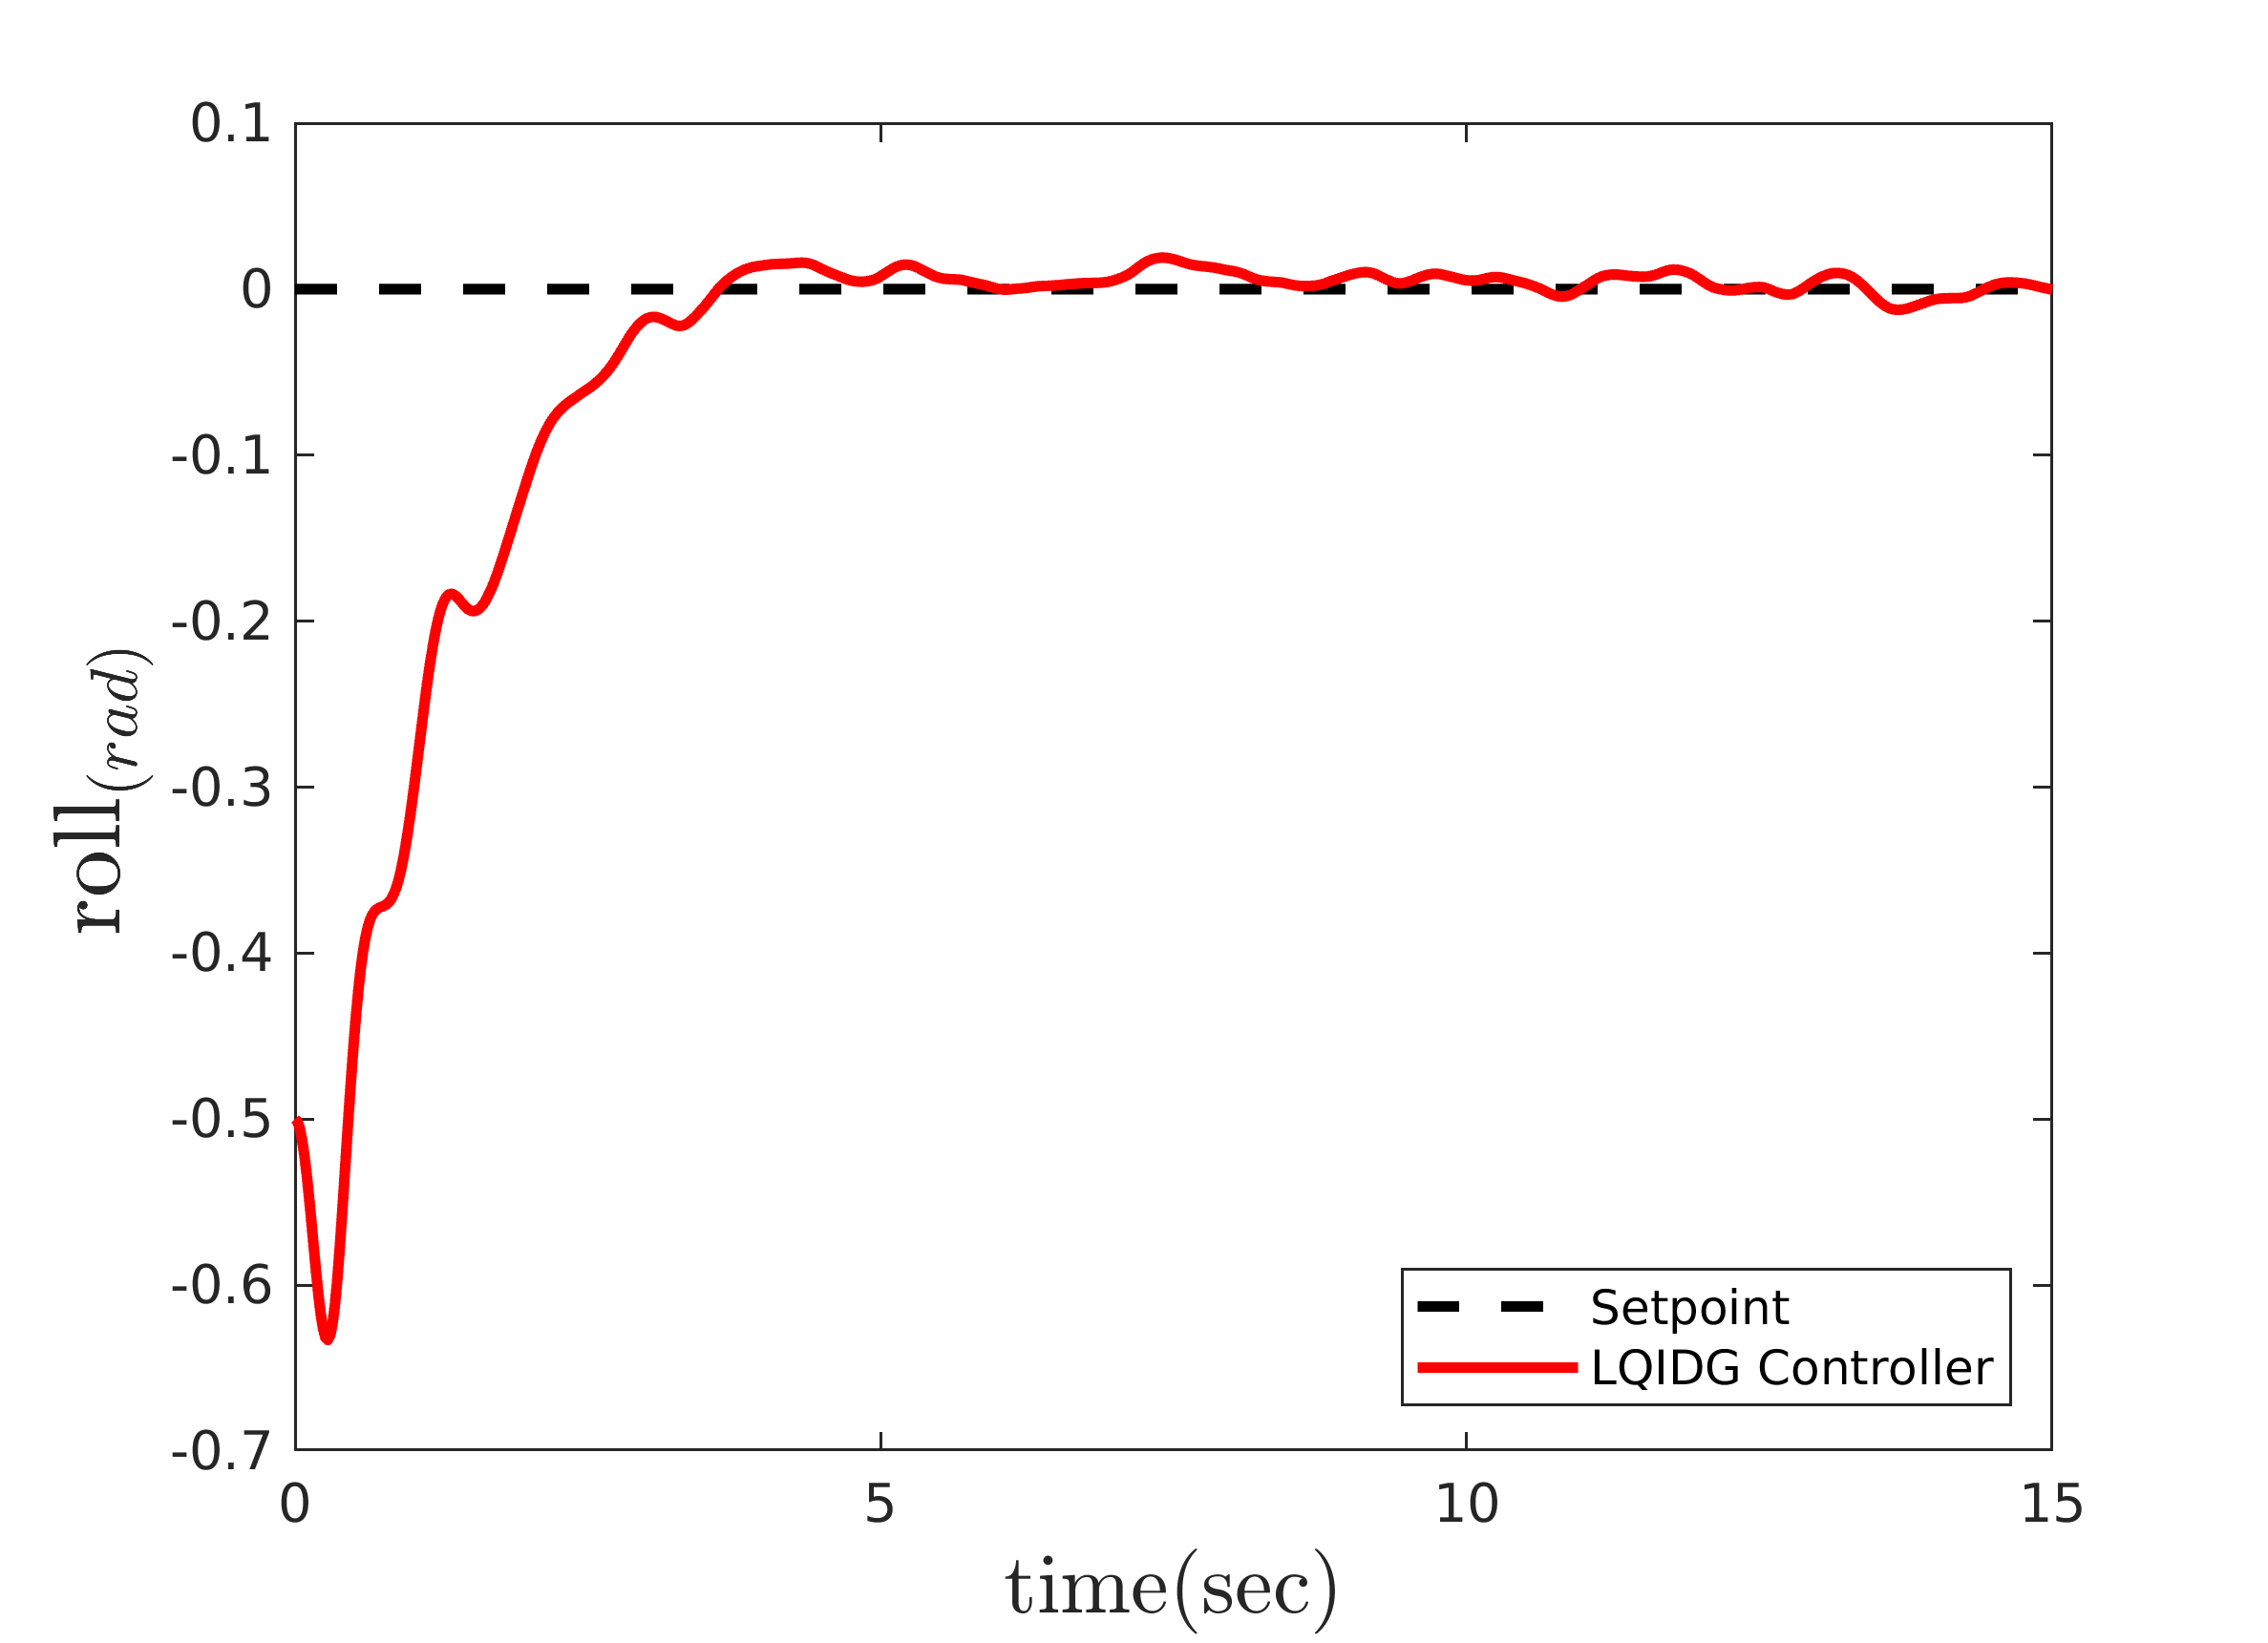
\includegraphics[width=12cm]{../Figures/MIL/LQIDG/3DOF/lqidg_roll.png}
	\centering
	\caption{عملكرد LQIDG در کنترل زاويه رول (تعقیب ورودی صفر)}
\end{figure}

\begin{figure}[H] 
	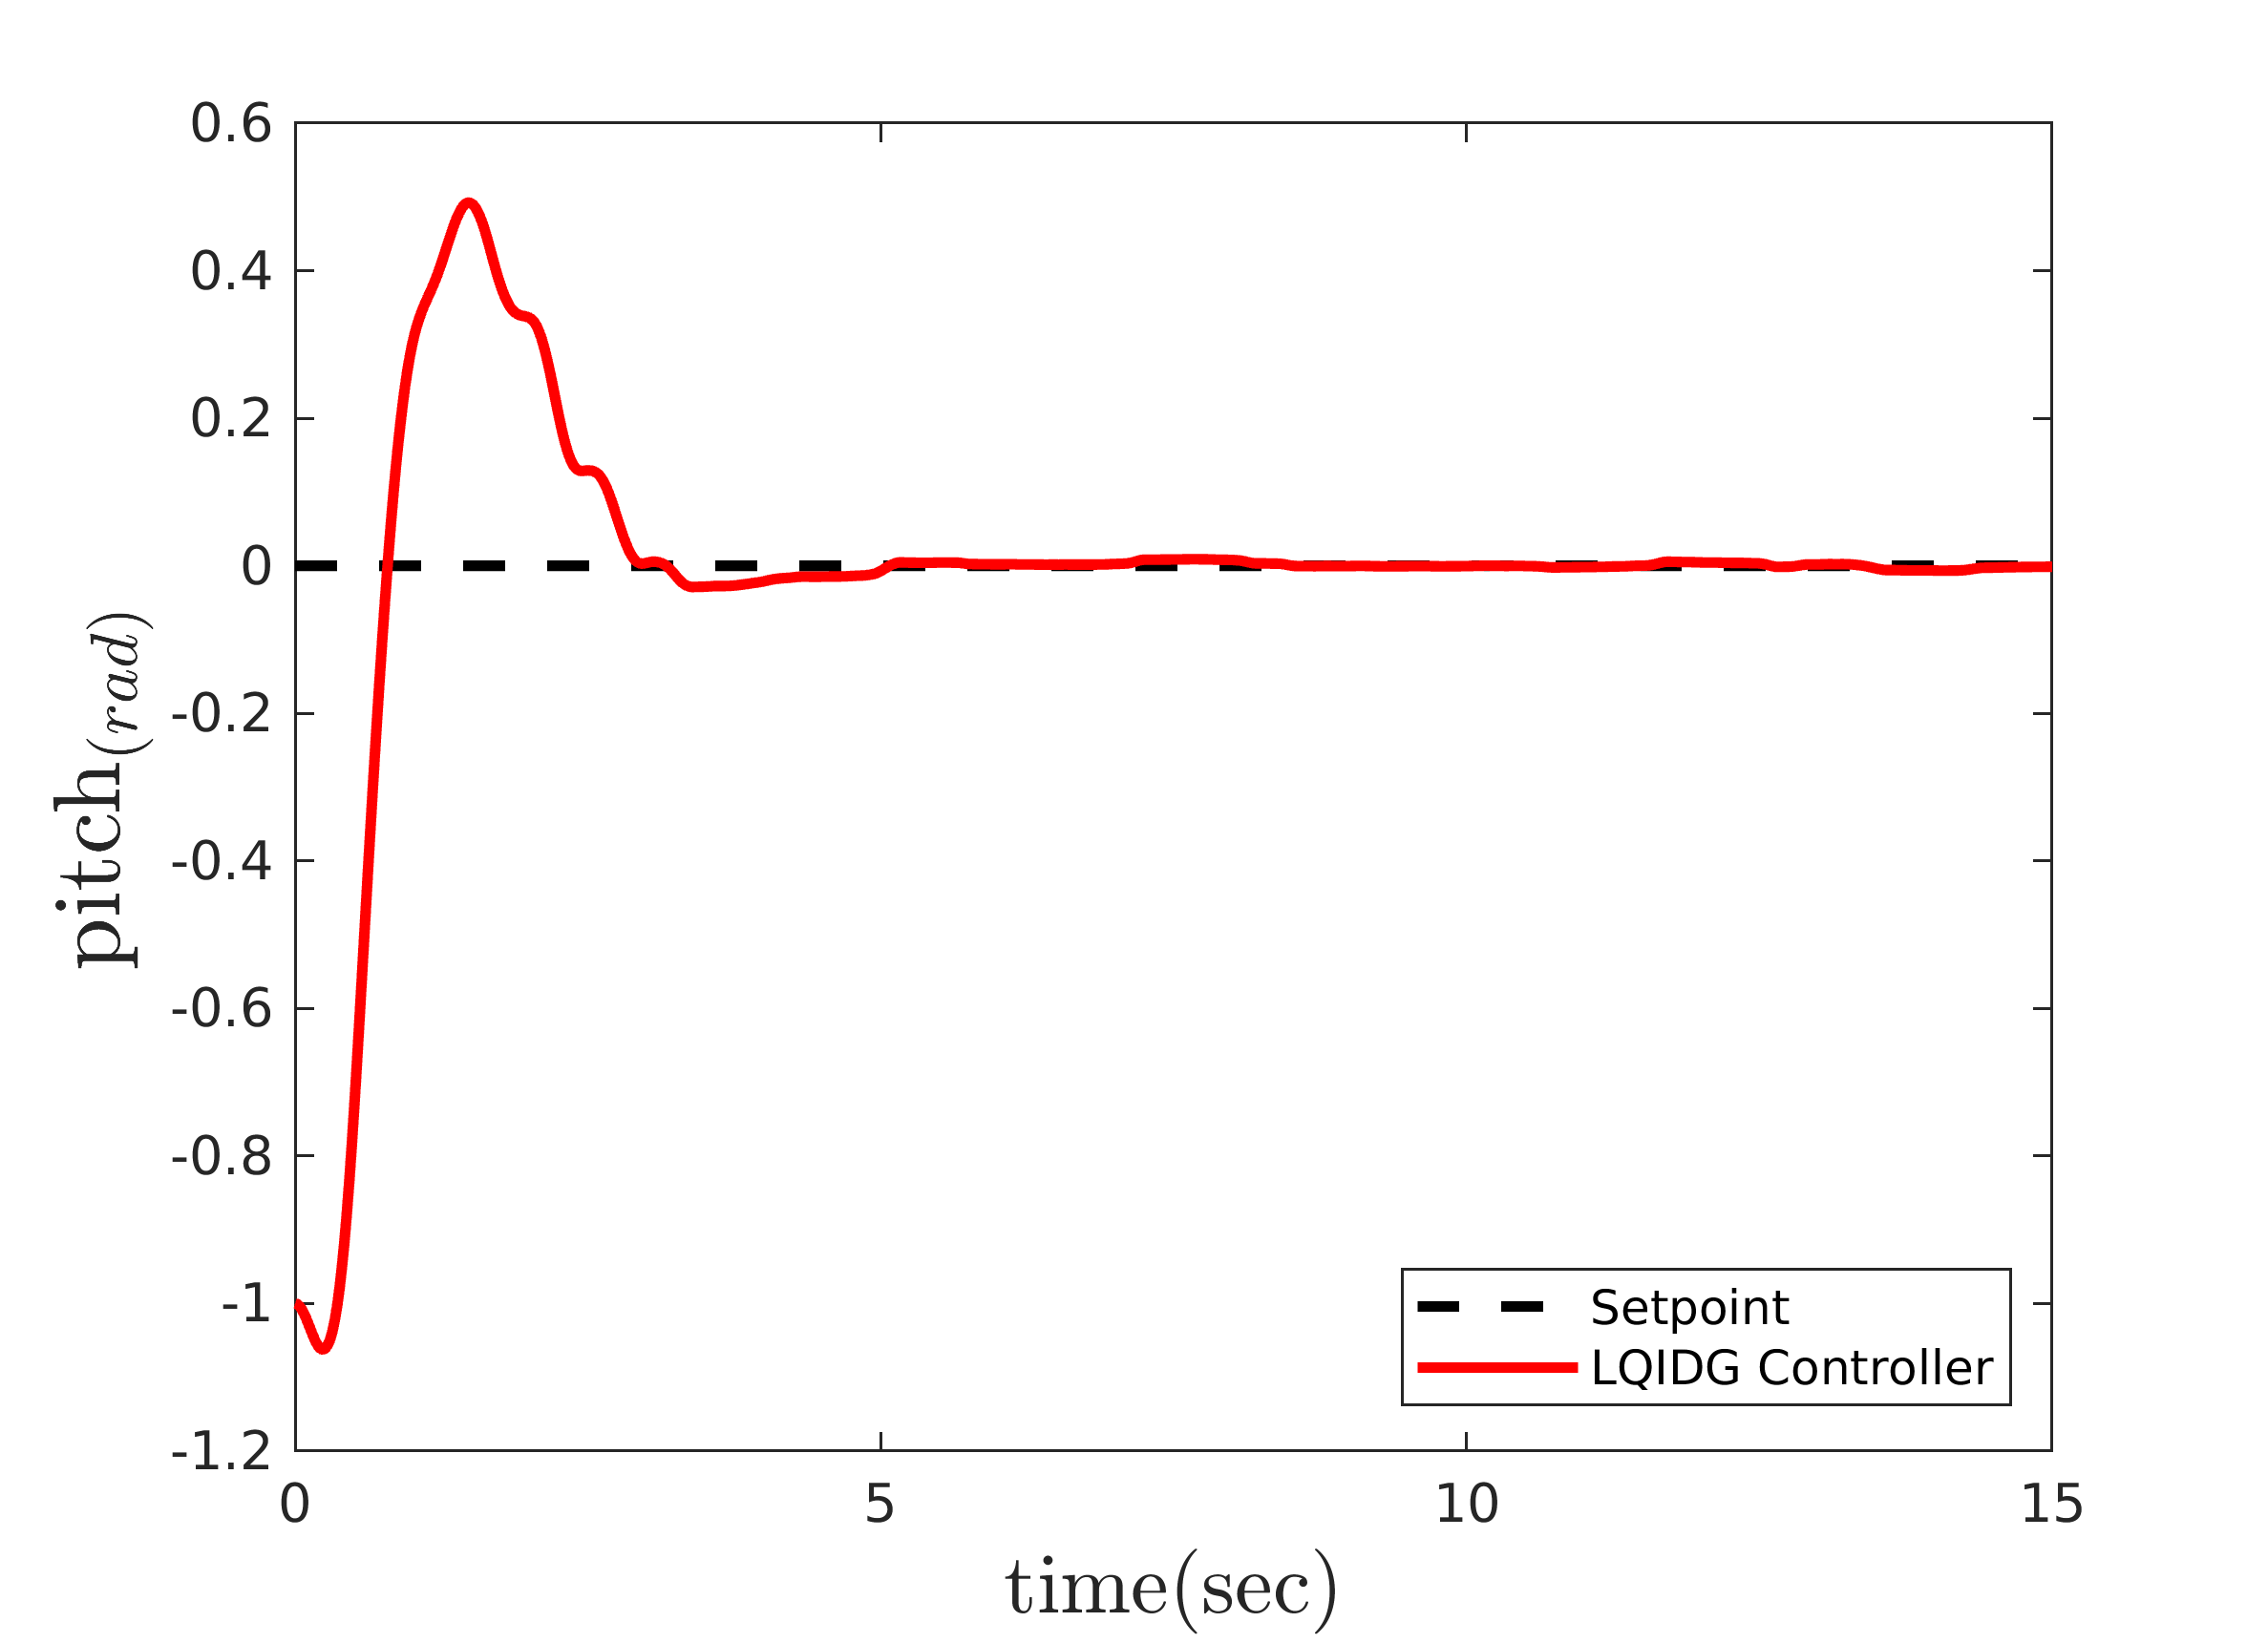
\includegraphics[width=12cm]{../Figures/MIL/LQIDG/3DOF/lqidg_pitch.png}
	\centering
	\caption{عملكرد LQIDG در کنترل زاويه پیچ (تعقیب ورودی صفر)}
\end{figure}

\begin{figure}[H]
	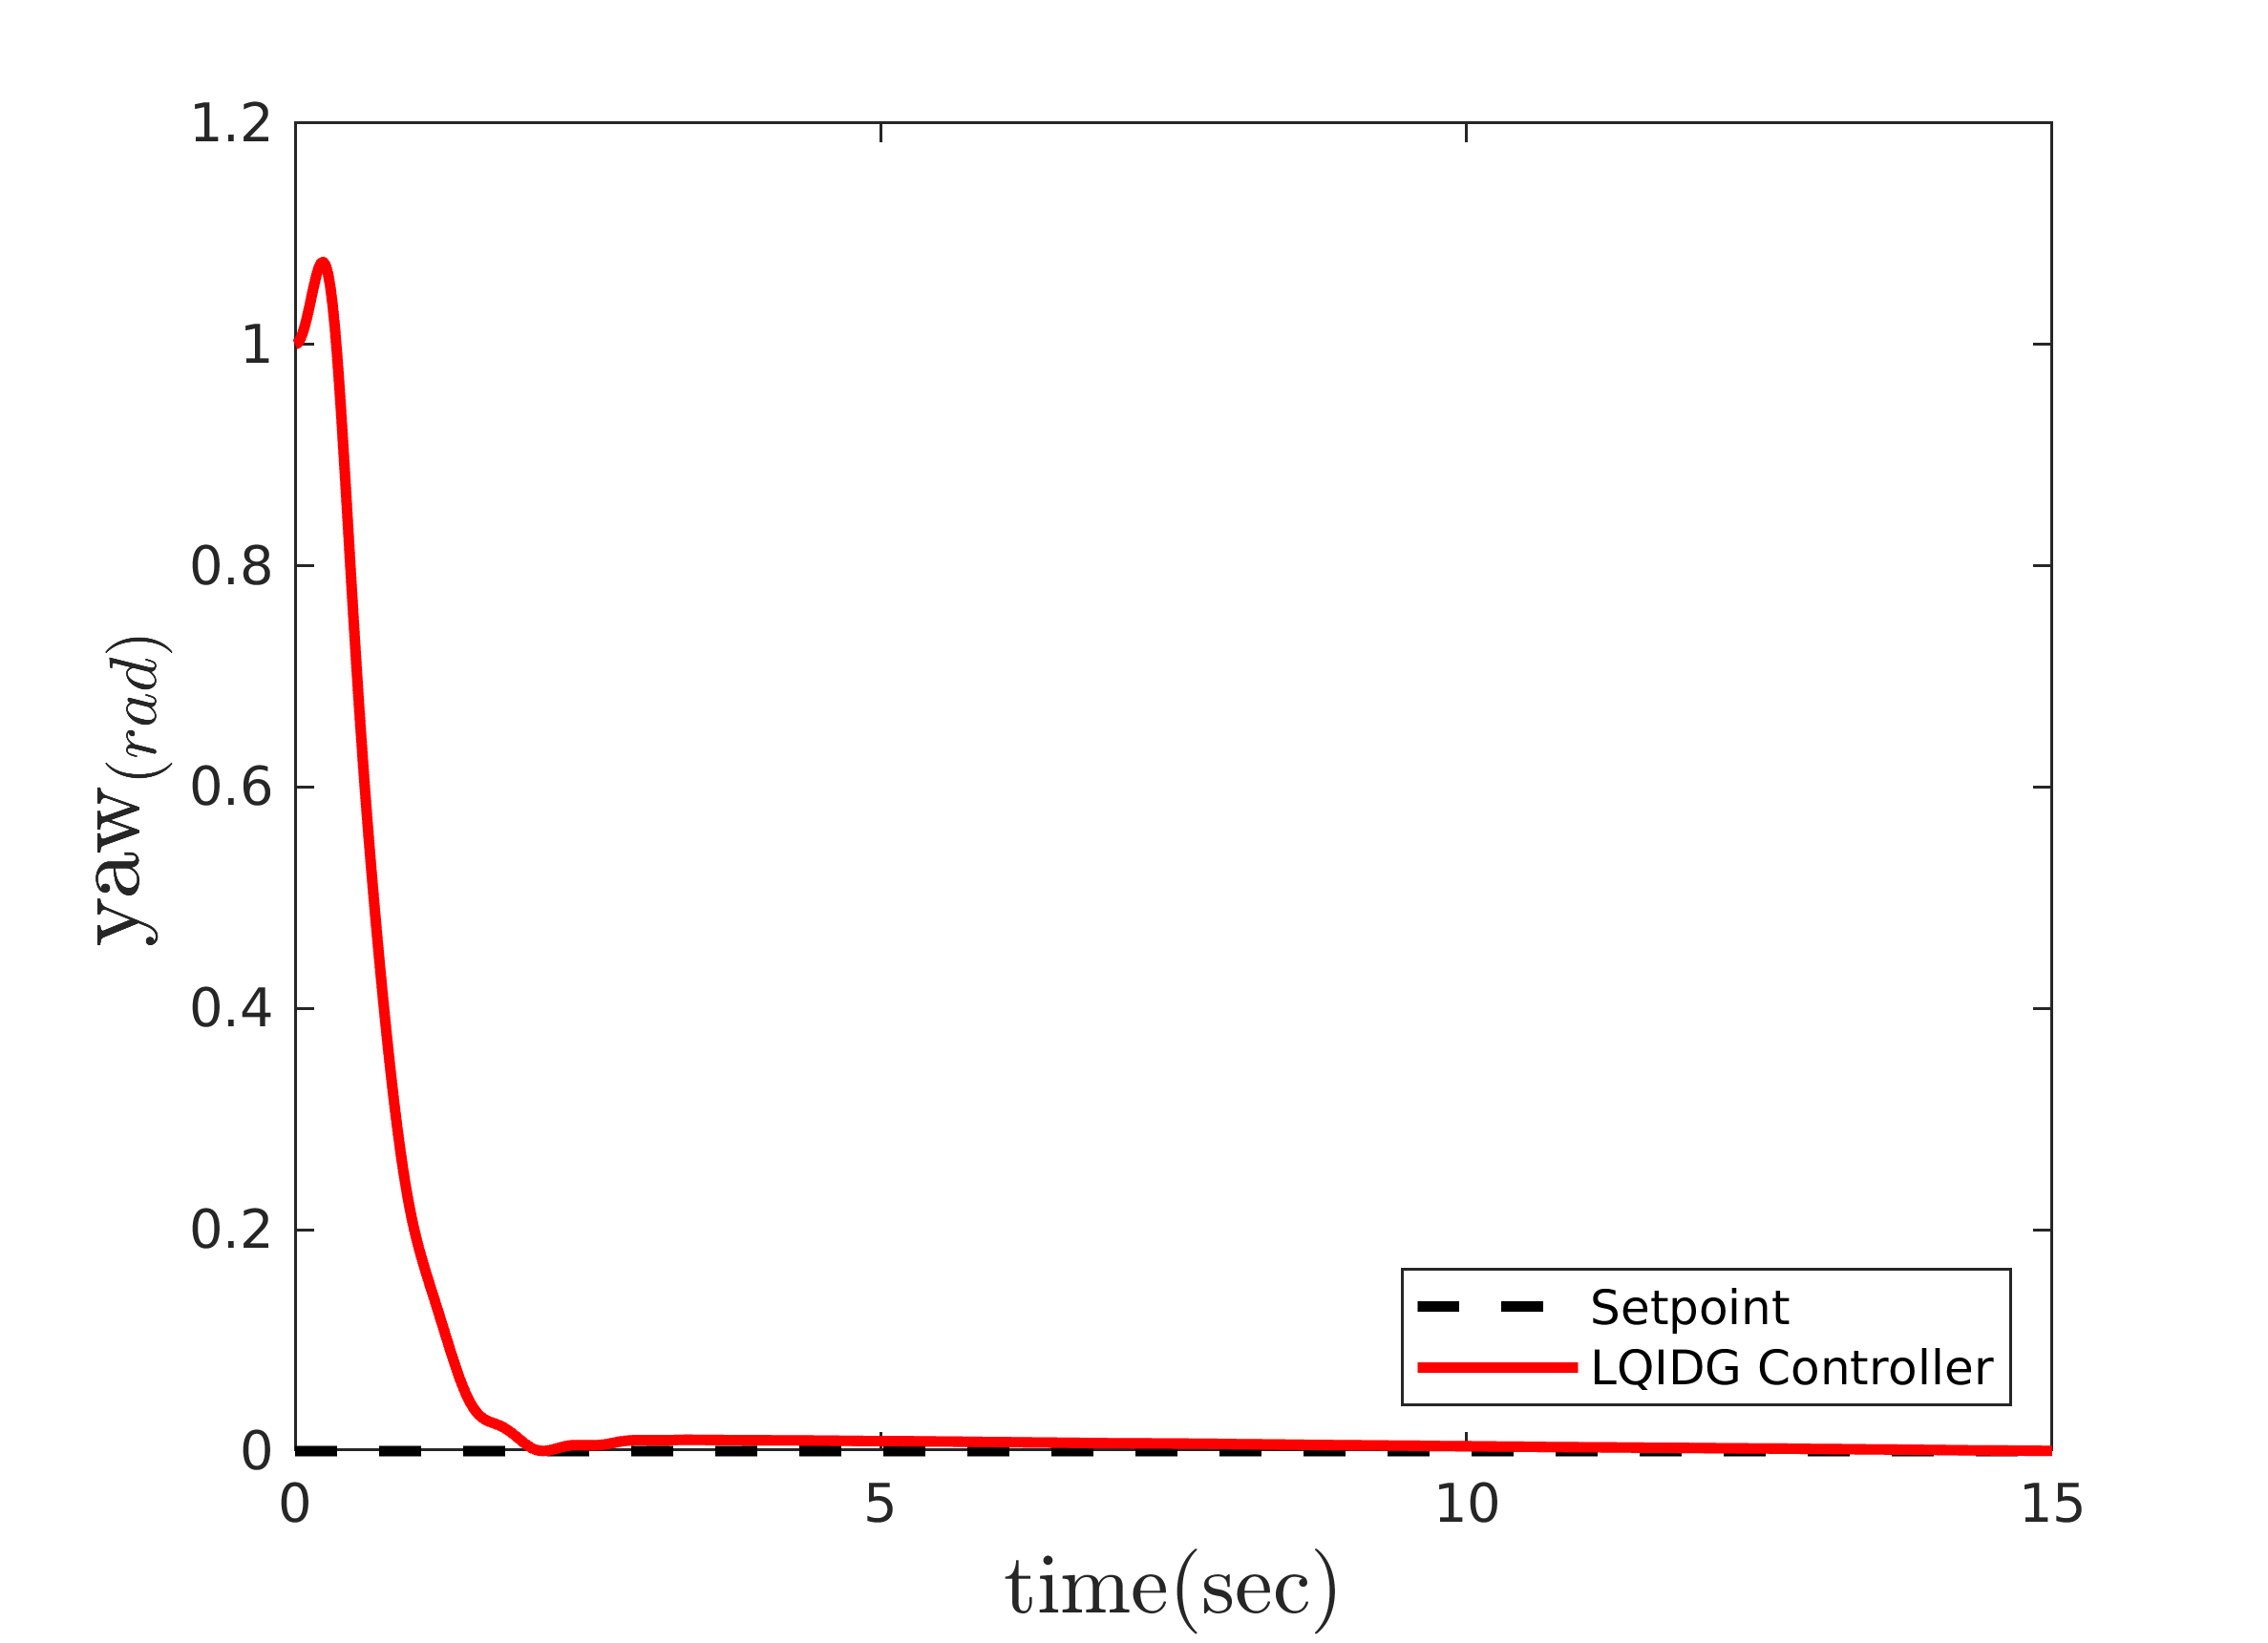
\includegraphics[width=12cm]{../Figures/MIL/LQIDG/3DOF/lqidg_yaw.png}
	\centering
	\caption{عملكرد LQIDG در کنترل زاويه یاو (تعقیب ورودی صفر)}
\end{figure}


%بر اساس خروجی شبیه‌سازی (شکل
%\ref{lqidg_roll_fig})
%،کانال رول در حضور کنترل‌کننده LQIDG در حدود پنج ثانیه و کانال پیچ در حدود هشت ثانیه به تعادل می‌رسد و خطای ماندگار آن در حدود صفر است.